\section{Problem statement}

\subsection{Biological generative model}
Here we suggest a model of the biological process such that given a set of reference genomes $G$ produces a query read (with phred values). There are no assumptions on the genomes and their (dis-)similarities.

Let $\{G_i\}$ be a set of $N$ given haploid genomes each with an associated occurrence probability $P_{occurence}(G_i)$. The large-scale variation between the genomes is assumed to be captured by $G$ being representative for different genome classes depending on the task.

Let there exists an infinite universe of genomes $U \supset G$ such that each genome has a defined probability to be observed: $P_{mutate}^{g \in G}(g' \in U) \sim 1 / d_{edit}(g, g')$. The edit distance $d_{edit}(\cdot,\cdot)$ function accounts for edit operations (insertions, deletion and substitutions) that are assumed to be a reasonable model for small-scale evolutional variation. The edit distance metric can account distinguish between different edit type or specific letter transformation.

Let $P_{start}$ be the probability of a read starting at position $start$ in the reference genome $g$ (note that the length may be slightly different than $\hat{g}$). Let there be a probabilistic process that introduces substitution changes to a read sequence. The substitution probabilities $phred_i$ are known for each read position $i$.

Generative model \fxnote{figure}: First, a genome $g$ is picked from $G$ according to $P_{occurence}$. Then $g$ is mutated into $\hat{g}$ according to $P_{mutate}$. Then a set of reads is sampled from $\hat{g}$: each fixed-length read $r$ is picked as a substring of $\hat{g}$ according to $P_{start}^g$. Finally, according to $P_{phred}$ technical errors are introduced to produce the read with errors $\hat{r}$. The generated set of reads is $\hat{R} = \{ (\hat{r},phred) \}$.

\subsection{Biological inference}
We formalize the problem of \textit{mapping} a set of reads (with phred values) to a set of genomes (or any structure $M$ capturing the information of a set of genomes). The goal is to find such a mapping of the reads that maximizes the probability of the set of reads being generated by the model. In other words,

\begin{align*}
	map_{\theta}(\hat{r}) &= \argmax_{\hat{g} \in U \wedge pos} P_{occ}(g) P_{mut}^{g}(\hat{g}) P_{start}^{g}(pos) P_{ph}(\hat{r}, r) \\
			\text{where}& \\
			& \theta = \langle P_{occ}, P_{mut}, P_{start}, P_{ph} \rangle \\
			& G - \text{is the finite set of the given reference genomes} \\
			& U - \text{is the infinite set of all possible genomes} \\
			& g = argmin_{g \in G} d_{edit}(\hat{g}, g), \\
			& r = g[pos : pos+len] \\
\end{align*}

\subsection{Boundary mapping conditions}
We postulate a set of properties that a mapping framework should preserve when combining different sources of uncertainty. 
As a verification of our approach, we impose the following boundary conditions where our mapping optimization task has to be equivalent to existing well known optimization criteria that are recognized by the community:
\begin{itemize}
	\item Assuming perfect phred values (all equal to 1, i.e. all bases are correctly read), no edit operations (no edit edges are added to the graph) and no discriminative variation probabilities (all equal to 1), the mapping task is equivalent to \textbf{exact mapping} (e.g. equivalen to vg\cite{VGtool} in the exact regime).
	\item Assuming perfect phred values and no edit operations: The graph accounts only for variation probabilities and the mapping is equivalent to \textbf{maximizing the path probability} generated by our model (by definition).
	\item Assuming perfect phred values and no discriminative variation probabilities: Mapping on such graph allows for edit operations and the mapping procedure \textbf{minimizes the edit distance}.
	\item Assuming no edit operations and no discriminative variation probabilities: Mapping is accounting only for the technical errors (i.e. phred values) and it is equivalent to \textbf{maximizing the probability that the query as a generative model will generate the path} (obviously, the path should be the same length as the query as indels are not permitted).
\end{itemize}

We show that our optimization task indeed satisfies all the stated boundary conditions and continuously and monotonically extrapolates between them. \fxwarning{justify, prove}

%\begin{figure}	
%	\centerline{
%		% Resize it to 5cm wide.
%		\resizebox{7cm}{!}{
%			\begin{tikzpicture}[
%			scale=0.5,
%			arrow/.style={->,shorten >=2pt,shorten <=2pt,>=stealth},
%			seq/.style={thick},
%			%virtual/.style={thick,densely dashed},
%			%trans/.style={thick,<->,shorten >=2pt,shorten <=2pt,>=stealth},
%			%classical/.style={thin,double,<->,shorten >=4pt,shorten <=4pt,>=stealth}
%			]
%			% TOP node
%			\draw[seq] (2cm,11em) -- (4cm,11em) node[midway,above] {references};
%			\draw[seq] (2.2cm,10.5em) -- (3.7cm,10.5em) node[midway,above] {};
%			\draw[seq] (1.7cm,10em) -- (3.8cm,10em) node[midway,above] {};
%			\draw[seq] (2cm,9.5em) -- (4.3cm,9.5em) node[midway,above] {};			
%			%
%			% LEFT column
%			\draw[arrow] (2.5cm,8em) -- (1cm,-2em) node[midway,left] {build graph};
%			\draw[seq] (0.5cm,-2em) node[left] {PNFA};
%			%
%			\draw[arrow] (1cm,-3em) -- (1cm,-12em) node[midway,left] {add edit edges};
%			\draw[seq] (0.5cm,-14em) node[left,align=right] {PNFA with\\edit edges};
%			%
%			% RIGHT column
%			\draw[arrow] (4cm,8em) -- (5.5cm,-2em) node[midway,right] {select};
%			\draw[seq] (4.5cm,-2em) -- (6cm,-2em) node[right] {sample};
%			%
%			\draw[arrow] (5.5cm,-3em) -- (5.5cm,-8em) node[midway,right] {edit};
%			\draw[seq] (4.5cm,-8em) -- (6cm,-8em) node[right] {mutated sample};
%			%
%			\draw[arrow] (5.5cm,-9em) -- (5.5cm,-15em) node[midway,right] {chop};
%			\draw[seq] (4.5cm,-15em) -- (6cm,-15em) node[right] {errorless read};
%			%
%			\draw[arrow] (5.5cm,-16em) -- (5.5cm,-21em) node[midway,right] {substitution errors};
%			\draw[seq] (4.5cm,-21em) -- (6cm,-21em) node[right] {read with phred};
%			%
%			% ARROWS in between
%			\draw[arrow] (2cm,-2em) -- (4cm,-2em) node[midway,left] {1};
%			\draw[arrow] (1.5cm,-14em) -- (4cm,-8em) node[midway,left] {2};
%			\end{tikzpicture}
%		}
%	}
%	\caption{Generative models. Going through 1 is equivalent as going through 2.}
%\end{figure}

\begin{figure*}
	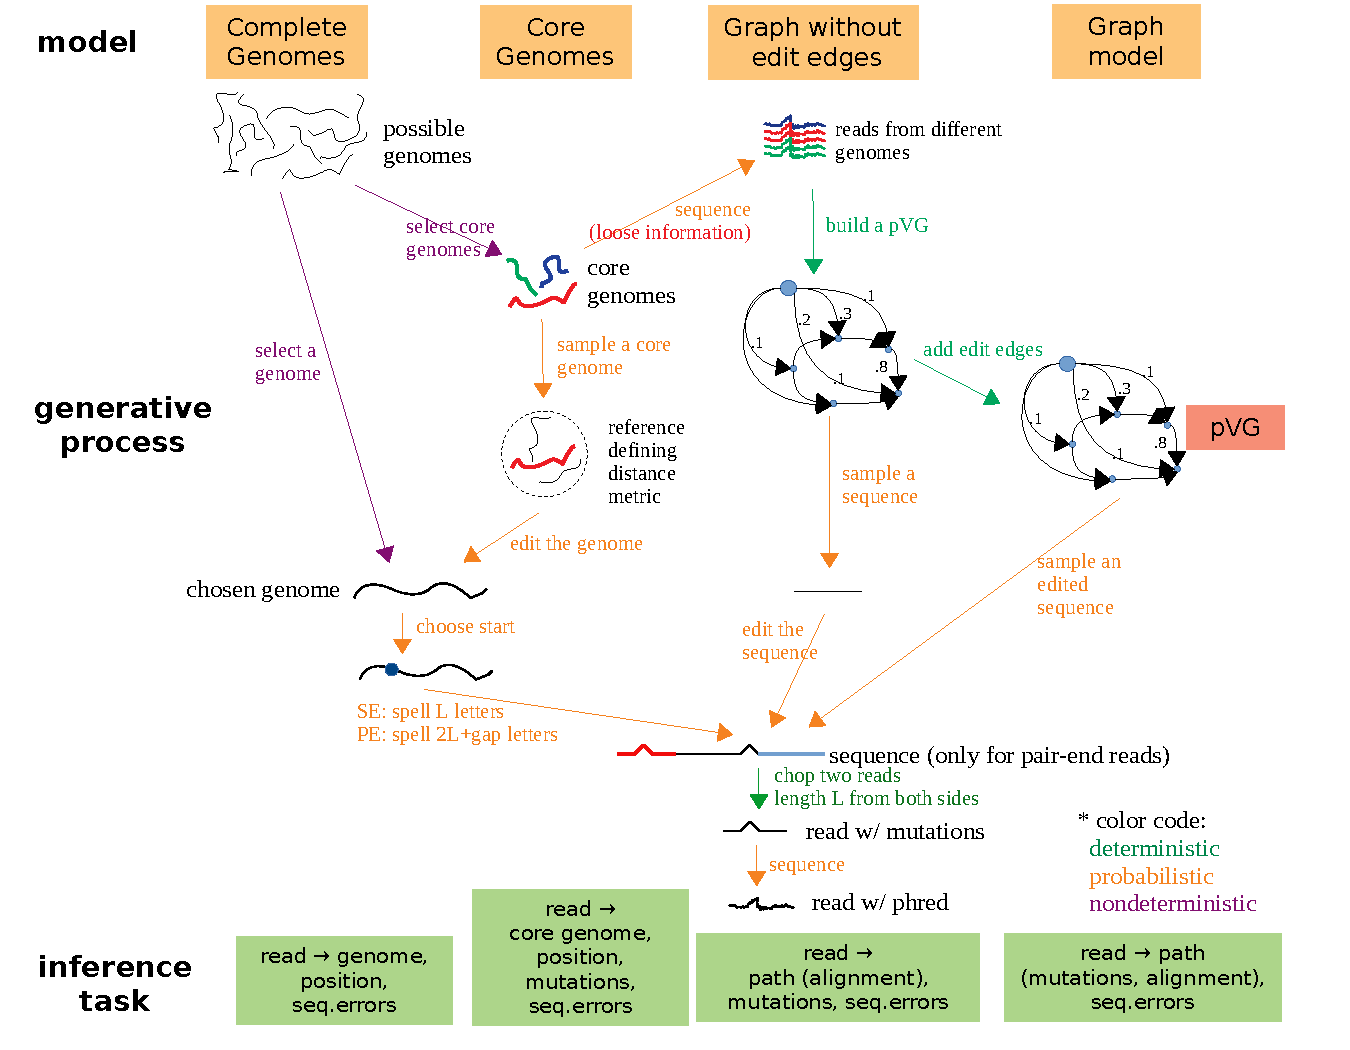
\includegraphics[width=\linewidth]{figures/models.pdf}
	\caption{Generative models and inference problems. Columns represent models. Colors capture the type of transitions: probabilistic, deterministic or nondeterministic}
	\label{fig:models}
\end{figure*}

After generating a sequence, technical noise is added according to a given phred profile.

